%!TEX root = ../chapter02.tex 
%----------------------------------------------------------------------------------------
%	
%----------------------------------------------------------------------------------------


%----------------------------------------------------------------------------------------
%	 
%----------------------------------------------------------------------------------------
 
\newpage 
\loadgeometry{marginlayout}  
\pagestyle{scrheadings} % Print headers again  
\KOMAoptions{
	headwidth=textwithmarginpar,
	headsepline=true,
	headsepline= 0.5pt,
	footwidth=textwithmarginpar,
	paper=A4,
	paper=portrait,
}     

\onehalfspacing 
\section{Identités remarquables}
 
\begin{theorem}[Le produit de conjuqués]
	Pour tout réels $a$ et $b\in\mathbb{R}$ :
	\begin{align*}
		(a+b)(a-b)&=a^2- b^2  
	\end{align*} 
	$(a-b)$ est le terme conjugué de $(a+b)$.\\
	$(a+b)$ est le terme conjugué de $(a-b)$
\end{theorem}
\begin{proof}\hfill
	 
\noindent \parbox{0.85\linewidth}{	
	$\begin{WithArrows}
		(a+b)(a-b) &=\\
		&= \rule{0pt}{1.1em}\\
		& = \rule{0pt}{1.1em}  \\
		& = \rule{0pt}{1.1em}  
	\end{WithArrows}$ 	
} \\
\null
\end{proof} 
\begin{example}\hfill 
	
\noindent \parbox{0.45\linewidth}{	
	$\begin{WithArrows}
		A & =(2x-3)(2x+3) \\
		&= \rule{0pt}{1.1em}\\
		& = \rule{0pt}{1.1em}  \\
		& = \rule{0pt}{1.1em}  
	\end{WithArrows}$ 	
}\hfill\parbox{0.45\linewidth}{	
$\begin{WithArrows}
	B & =(\sqrt{5}+2)(\sqrt{5}-2) \\
	&= \rule{0pt}{1.1em}\\
	& = \rule{0pt}{1.1em}  \\
	& = \rule{0pt}{1.1em}  
\end{WithArrows}$ 
\marginnote{
\begin{tBox}[leftline=false]
	$(ab)^2  = a^2 b^2$
\end{tBox}
}[0mm] 	
}
\end{example} 
\begin{marginfigure}
	\begin{tikzpicture}[scale=0.80]
		\tkzDefPoint(0,0){O}
		\tkzDefPoint(2.5,0){A}
		\tkzDefPoint(4,0){A'}
		\tkzDefSquare(O,A)\tkzGetPoints{B}{C}
		\tkzDefSquare(O,A')\tkzGetPoints{B'}{C'}
		\tkzDefPoint(4,2.5){D}
		\tkzDefPoint(2.5,4){D'}
		\tkzDrawSquare[color=black](O,A)
		\tkzDrawSquare[color=black](B,D)
		\tkzDrawSquare[color=black, line width=2pt](O,A')
		\tkzLabelSegment[below](O,A){$a$}
		\tkzLabelSegment[below](A',A){$b$}
		\tkzLabelSegment[left](O,C){$a$}
		\tkzLabelSegment[left](C,C'){$b$}
	\end{tikzpicture}
	\caption{Illustration géométrique du carré de la somme de nombres positifs $a\geqslant 0$ et $b\geqslant 0$}
	\label{chapitre02:figure:carresomme}
\end{marginfigure}   
\begin{theorem}[Carré de somme]
	Pour deux nombres $a\neq 0$ et $b\neq 0$ :
	\begin{align*}
		(a+b)^2 &= a^2+2ab+b^2  & 	(a-b)^2 &= a^2-2ab+b^2   
	\end{align*} 
\end{theorem}
\begin{proof}\hfill 

\noindent \parbox{0.45\linewidth}{	
	$\begin{WithArrows}
	(a+b)^2 &= (a+b)(a+b) \\
		&= \rule{0pt}{1.1em}\\
		& = \rule{0pt}{1.1em}  \\
		& = \rule{0pt}{1.1em}  
	\end{WithArrows}$ 	
}\hfill\parbox{0.45\linewidth}{	
	$\begin{WithArrows}
	(a-b)^2 &=  (a-b)(a-b) \\
		&= \rule{0pt}{1.1em}\\
		& = \rule{0pt}{1.1em}  \\
		& = \rule{0pt}{1.1em}  
	\end{WithArrows}$ 	
} \\
\null	
%	\begin{align*}
%		(a+b)^2 &= (a+b)(a+b)  & 	(a-b)^2 &=  (a-b)(a-b) \\
%		&=   & 	 &=  \\
%		&=   & 	 &=   
%	\end{align*} 
\end{proof} 
\begin{example} \hfill 
	\begin{multicols}{2}
		\begin{enumerate}[label={$\Alph*(x)=$},leftmargin=*]
			\item $(2x-3)^2$  
			\item $(2x+3)^2$ 
		\end{enumerate}
	\end{multicols}
\end{example}
%\begin{remark} Carrés de produits. Pour tous réels $a\neq 0$ et $b\neq 0$ :
%	\begin{align*} 
%		(ab)^2 &= a^2 b^2 & \left(\frac{a}{b}\right)^2 &= \frac{a^2}{b^2} 
%	\end{align*}  
%\end{remark}







%----------------------------------------------------------------------------------------
%	EXERCICES
%----------------------------------------------------------------------------------------

\newpage 
\loadgeometry{widelayout}  
\pagestyle{scrheadings} % Print headers again  
\KOMAoptions{
	headwidth=textwithmarginpar,
	headsepline=true,
	headsepline= 0.5pt,
	footwidth=textwithmarginpar,
} 
\onehalfspacing
\subsection{Exercices : identités remarquables}




\begin{exercise} \label{chap02:exo:identite:niveau1}
	$x\in\mathbb{R}$. Développer à l'aide de l'identité remarquable adaptée :
	\begin{multicols}{3}
		\begin{enumerate}[label={$\Alph*=$},left= 0pt]
			\item $(3x+5)^2$  
			\item $(x-8)(x+8)$ 
			\item $(1+\sqrt{5})^2$
			\item $(\sqrt{2}-1)^2$
			\item $(2\sqrt{3}-5)^2$
			\item $2(4x-3)^2$  
			\item $(6x-5)(6x+5)$  
			\item $2(3x-\sqrt{5})^2$  
			\item $(9\sqrt{2}-7)(9\sqrt{2}+7)$
%			\item $ (5\sqrt{8}-2\sqrt{7})(5\sqrt{8}+2\sqrt{7})$   
		\end{enumerate}
	\end{multicols}
\end{exercise}

\begin{exercise} \label{chap02:exo:identite:niveau2} Même consignes. 
	\begin{multicols}{2}
		\begin{enumerate}[label={$\Alph*(x)=$}, align=left] 
			\item $(5x+\sqrt{3})^2-x^2$
			\item  $(6x+9)^2-(x-5)(x-5)$ 
			\item $(5x+2)^2-(2x+3)(2x-3)$
			\item  $(3x+2)(3x-2)- 2(x-5)^2$ 
		\end{enumerate}
	\end{multicols}
\end{exercise}
\begin{example}[Je fais] Transformer les fractions suivantes, pour obtenir une fraction égale ayant un dénominateur entier : \hfill 
	
\noindent\hfill\parbox{0.30\linewidth}{	
$\begin{WithArrows}
		\frac{7}{3\sqrt{5}}& = \frac{7\times \sqrt{5} }{3\sqrt{5}\times \sqrt{5}}  \\
		&= \frac{7\sqrt{5}}{\sqrt{25}} \\
		& = \frac{7\sqrt{5}}{5}  \\ 
		& \rule{0pt}{1.2em} %= \rule{0pt}{1.1em}  
	\end{WithArrows}$ 	
} \hfill\parbox{0.30\linewidth}{	
$\begin{WithArrows}
	\frac{3}{\sqrt{12}} &= \\ % \frac{3\times\sqrt{12}}{\sqrt{12}\times\sqrt{12}} \\
	&= \rule{0pt}{1.2em}  \\ %\frac{3\sqrt{12}}{12} \\
	& = \rule{0pt}{1.2em}  \\ %\frac{3\sqrt{4}\sqrt{3}}{12}  \\
	& = \rule{0pt}{1.2em}   % \frac{6\sqrt{3}}{12}= \frac{\sqrt{3}}{2} 
\end{WithArrows}$ 	
}  \hfill\parbox{0.30\linewidth}{	
$\begin{WithArrows}
\frac{4}{\sqrt{8}} &= \rule{0pt}{1.2em} \\ %\frac{4\times\sqrt{8}}{\sqrt{8}\times\sqrt{8}} \\
	&=\rule{0pt}{1.2em}  \\ % \frac{4\times\sqrt{4}\sqrt{2}}{8}\\
	& =\rule{0pt}{1.2em} \\ %\frac{8\sqrt{2}}{8}  \\
	& = \rule{0pt}{1.2em} % \sqrt{2}
\end{WithArrows}$
}  
\end{example} 
\begin{exercise}[\cancel{\faCalculator} À vous]\label{chap02:exo:identite:radicaux1} Mêmes consignes.
	\begin{multicols}{5}
	\begin{enumerate}[label={$\Alph*=$},leftmargin=*]
		\item $\frac{5}{\sqrt{7}}$
		\item $\frac{10}{\sqrt{6}}$
		\item $\frac{2}{\sqrt{10}}$
		\item $\frac{\sqrt{3}}{\sqrt{5}}$
		\item $\frac{\sqrt{3}}{\sqrt{7}}$
		\item $\frac{-\sqrt{9}}{\sqrt{3}}$
		\item $\frac{14}{3\sqrt{7}}$
		\item $\frac{7}{2\sqrt{3}}$
		\item $\frac{\sqrt{5}}{\sqrt{10}}$
		\item $\frac{\sqrt{12}}{2}$
	\end{enumerate}
\end{multicols}
\end{exercise}
\begin{example}[Je fais] Mêmes consignes. \hfill 

\noindent\hfill\parbox{0.32\linewidth}{	
	$\begin{WithArrows}
		\frac{3}{2+\sqrt{3}}& = \rule{0pt}{1.6em} \\
		&= \rule{0pt}{1.6em} \\
		& =\rule{0pt}{1.6em}  \\ 
		&= \rule{0pt}{1.6em} %= \rule{0pt}{1.1em}  
	\end{WithArrows}$ 	
} \hfill\parbox{0.32\linewidth}{	
	$\begin{WithArrows}
		\frac{4}{\sqrt{5}-2} &=  \rule{0pt}{1.6em} \\ % \frac{3\times\sqrt{12}}{\sqrt{12}\times\sqrt{12}} \\
		&= \rule{0pt}{1.6em}  \\ %\frac{3\sqrt{12}}{12} \\
		& = \rule{0pt}{1.6em}  \\ %\frac{3\sqrt{4}\sqrt{3}}{12}  \\
		& = \rule{0pt}{1.6em}   % \frac{6\sqrt{3}}{12}= \frac{\sqrt{3}}{2} 
	\end{WithArrows}$ 	
}  \hfill\parbox{0.32\linewidth}{	
	$\begin{WithArrows}
		\frac{6}{\sqrt{5}-\sqrt{2}} &= \rule{0pt}{1.6em} \\ %\frac{4\times\sqrt{8}}{\sqrt{8}\times\sqrt{8}} \\
		&=\rule{0pt}{1.6em}  \\ % \frac{4\times\sqrt{4}\sqrt{2}}{8}\\
		& =\rule{0pt}{1.6em} \\ %\frac{8\sqrt{2}}{8}  \\
		& = \rule{0pt}{1.6em} % \sqrt{2}
	\end{WithArrows}$
}  
\end{example} 
\begin{exercise}[À vous] \label{chap02:exo:identite:radicaux2} Mêmes consignes.
	\begin{multicols}{4}
		\begin{enumerate}[label={$\Alph*=$\rule{0pt}{1.8em}},leftmargin=*]
			\item  $\frac{2}{4+\sqrt{3}}$
			\item $\frac{5}{7-\sqrt{5}}$
			\item $\frac{10}{5+\sqrt{2}}$
			\item $\frac{15}{\sqrt{7}-5}$
			\item $\frac{4}{3\sqrt{2}-10}$
			\item $\frac{3}{4-7\sqrt{3}}$
			\item $\frac{4\sqrt{2}}{\sqrt{2}-1}$
			\item $\frac{\sqrt{3}-\sqrt{2}}{\sqrt{3}+\sqrt{2}}$
		\end{enumerate}
	\end{multicols}
\end{exercise}



\begin{tBox}[frametitle={Transformer les fractions pour rendre le dénominateur entier} ] 
	\begin{description}
		\item[Cas 1] Le dénominateur est un produit ayant pour facteur $\sqrt{a} $.  
		On multiplie numérateur et le dénominateur par $\sqrt{a} $. 
		\item[Cas 2] Le dénominateur est de la forme $a\pm\sqrt{b}$  ( ou $\sqrt{a}\pm\sqrt{b}$ ) on multiplie numérateur et dénominateur par le conjugué.  
	\end{description}
\end{tBox}


\begin{exercise}[\cancel{\faCalculator}]Dans la figure ci-contre, $AEFD$, $EGHF$ et $GBJI$ sont des carrés. \hfill 
	
	\noindent\parbox[position=t]{0.3\linewidth}{  \centering
	\begin{tikzpicture}[scale=2.0] 
		\tkzSetUpPoint[size=3, fill=black]
		\tkzfctset{tan style/.style={->,>=latex, color=red, line width=1.2pt}}   
		\tkzSetUpLine[line width= 1.2pt, add=.5 and .5] 
		
		\tkzDefPoint(0,0){A} 
		\tkzDefPoint(5**0.5,0){B} 
		\tkzDefPoint(5**0.5,-1){C} 
		\tkzDefPoint(0,-1){D} 
		\tkzDrawPolygon[](A,B,C,D)
		
		\tkzDefPoint(1,0){E}
		\tkzDefPoint(1,-1){F}
		
		\tkzDefPoint(2,0){G}
		\tkzDefPoint(2,-1){H}
		
		\tkzDefPoint(2,2-5**0.5){I}
		\tkzDefPoint(5**0.5,2-5**0.5){J}
		
		\tkzDrawSegment[dim={\scriptsize $\sqrt{5}$,+25pt,}](A,B)
		\tkzDrawSegment[dim={\scriptsize $1$,-25pt,}](A,D)
		\tkzDrawSegments[dashed](E,F G,H)
		\tkzDrawPolygon[fill=gray!20](I,J,C,H)  
		\tkzLabelPoint[above left](A){\scriptsize$A$}
		\tkzLabelPoint[above right](B){\scriptsize$B$} 
		\tkzLabelPoint[below right](C){\scriptsize$C$} 	
		\tkzLabelPoint[below](D){\scriptsize$D$} 
		\tkzLabelPoint[above](E){\scriptsize$E$} 
		\tkzLabelPoint[below](F){\scriptsize$F$} 
		\tkzLabelPoint[above](G){\scriptsize$G$} 
		\tkzLabelPoint[below](H){\scriptsize$H$}  
		\tkzLabelPoint[left](I){\scriptsize$I$} 
		\tkzLabelPoint[right](J){\scriptsize$J$} 
	\end{tikzpicture}
}\hfill 
\parbox[position=r]{0.60 \linewidth}{    
\begin{enumerate}[label=\arabic*),leftmargin=*]
	\item Exprimer les dimensions du rectangle $IJCH$ en fonction de $\sqrt{5}$
	\item Démontrer que $\frac{IH}{IJ}=\sqrt{5}$.
	\item Quel est le rapport de réduction entre les rectangles $ABCD$ et $IJCH$ ?
\end{enumerate} 
} 
\end{exercise}
\begin{exercise}[classique] \hfill 
	\begin{enumerate}[label={\alph*)},leftmargin=*]
			\item Développer simplifier et réduire $(3+5\sqrt{2})^2$.  En déduire une écriture simplifiée de $\sqrt{59+30\sqrt{2}}$.
			\item Développer simplifier et réduire  $(2-\sqrt{5})^2$. En déduire une écriture simplifiée de $\sqrt{9-4\sqrt{5}}$.
	\end{enumerate}
\end{exercise} 
\vfill 
\begin{proof}[solution de l'exercice \ref{chap02:exo:identite:niveau1}]
\begin{pycode}
from re import sub
import sympy as sp

x, y, z, t = sp.symbols('x y z t')
k, m, n = sp.symbols('k m n', integer=True)
f, g, h = sp.symbols('f g h', cls=sp.Function)

# Create a list of functions to include in the table
funcs = ['(3*x+5)**2',
'(x-8)*(x+8)',
'(1+sp.sqrt(5))**2',
'(sp.sqrt(2)-1)**2',
'(2*sp.sqrt(3)-5)**2',
'2*(4*x-3)**2',
'(6*x-5)*(6*x-5)',
'2*(3*x-sp.sqrt(5))**2',
'(9*sp.sqrt(2)-7)*(9*sp.sqrt(2)+7)'
]
n=0
L=['A', 'B', 'C', 'D', 'E', 'F', 'G', 'H', 'I'  ]
for func in funcs:
	# Put in some vertical space when switching to arc and hyperbolic funcs 
	developpee =  eval('sp.expand('+ func +')') 
	print( "$"+L[n] + "=" + sp.latex( eval('developpee') )  + r'$; ' ) 
	n     = n + 1 
\end{pycode}
\end{proof}
\begin{proof}[solution de l'exercice \ref{chap02:exo:identite:niveau2}]
\begin{pycode}
from re import sub
import sympy as sp

x, y, z, t = sp.symbols('x y z t')
k, m, n = sp.symbols('k m n', integer=True)
f, g, h = sp.symbols('f g h', cls=sp.Function)

# Create a list of functions to include in the table
funcs = ['(5*x+sp.sqrt(3))**2-x**2',
'(6*x+9)**2-(x-5)*(x+5)',
'(5*x+2)**2-(2*x+3)*(2*x-3)',
'(3*x+2)*(3*x-2)-2*(x-5)**2' 
]
n=0
L=['A', 'B', 'C', 'D', 'E', 'F', 'G', 'H', 'I'  ]
for func in funcs:
	# Put in some vertical space when switching to arc and hyperbolic funcs 
	developpee =  eval('sp.expand('+ func +')') 
	print( "$"+L[n] + "(x) =" + sp.latex( eval('developpee') )  + r'$; ' ) 
	n     = n + 1 
\end{pycode}
\end{proof}
\begin{proof}[solution de l'exercice \ref{chap02:exo:identite:radicaux1}]
\begin{pycode}
from re import sub
import sympy as sp

x, y, z, t = sp.symbols('x y z t')
k, m, n = sp.symbols('k m n', integer=True)
f, g, h = sp.symbols('f g h', cls=sp.Function)

# Create a list of functions to include in the table
funcs = ['5/(sp.sqrt(7))',
'10/(sp.sqrt(6))',
'2/(sp.sqrt(10))',
'(sp.sqrt(3))/(sp.sqrt(7))',
'(-sp.sqrt(9))/(sp.sqrt(3))',
'(14)/(3*sp.sqrt(7))',
'(7)/(2*sp.sqrt(7))',
'(sp.sqrt(5))/(sp.sqrt(10))',
'(sp.sqrt(12))/(2)'
]
n=0
L=['A', 'B', 'C', 'D', 'E', 'F', 'G', 'H', 'I'  ]
for func in funcs:
	# Put in some vertical space when switching to arc and hyperbolic funcs
	simplifiee =  eval('sp.radsimp('+ func +')')
	print( "$"+L[n] + " =" + sp.latex( eval('simplifiee') )  + r'$; ' )
	n     = n + 1
\end{pycode}
\end{proof}	
\begin{proof}[solution de l'exercice \ref{chap02:exo:identite:radicaux2}]
	\begin{pycode}
from re import sub
import sympy as sp

x, y, z, t = sp.symbols('x y z t')
k, m, n = sp.symbols('k m n', integer=True)
f, g, h = sp.symbols('f g h', cls=sp.Function)

# Create a list of functions to include in the table
funcs = ['2/(4+sp.sqrt(3))',
'5/(7-sp.sqrt(5))',
'10/(5+sp.sqrt(2))',
'15/( sp.sqrt(7)-5)',
'4/(3*sp.sqrt(2)-10)',
'3/(4-7*sp.sqrt(3))',
'(4*sp.sqrt(2))/(sp.sqrt(2)-1)',
'(sp.sqrt(3)-sp.sqrt(2))/(sp.sqrt(3)-sp.sqrt(2))' 
]
n=0
L=['A', 'B', 'C', 'D', 'E', 'F', 'G', 'H', 'I'  ]
for func in funcs:
	# Put in some vertical space when switching to arc and hyperbolic funcs
	simplifiee =  eval('sp.radsimp('+ func +')')
	print( "$"+L[n] + " =" + sp.latex( eval('simplifiee') )  + r'$; ' )
	n     = n + 1
\end{pycode}
\end{proof}
%----------------------------------------------------------------------------------------
%	 
%---------------------------------------------------------------------------------------- 